% Provenance (never printed): cycle 3 "La planete Terre" (the shaping of
% landscapes: erosion, transport and deposition by running water; rivers
% from source to mouth; floods); see sources/book1/PROVENANCE.md.
% Book 1, grade 5, chapter 1.
\chapter{पानी ज़मीन को आकार देता है}\label{ch:g5:water-shapes-the-land}

पूरी रात तूफ़ान स्कूल की छत पर ढोल बजाता रहा। सुबह आसमान साफ़ हो रहा है, और
लीना और टॉम खेल के मैदान के पीछे की छोटी धारा की ओर दौड़ते हैं। कल वह साफ़ और
शांत थी: वे उसकी तली के \omterm{def:g3:stones-pebbles-sand:pebble}{कंकड़} गिन सकते थे। आज वह चौड़ी, तेज़ और भूरी है, दूधिया
चॉकलेट के रंग की। वह टहनियाँ और पत्तियाँ बहा रही है, और कुछ ऐसा भी जिसे वे एक-एक
करके नहीं देख सकते: \omterm{def:g3:stones-pebbles-sand:sand}{कीचड़} और \omterm{def:g3:stones-pebbles-sand:sand}{रेत}, जो उसके किनारों से और ऊपर की ओर के खेतों से
उखाड़ी गई
है।

``यह सारा \omterm{def:g3:stones-pebbles-sand:sand}{कीचड़} कहाँ जा रहा है?'' टॉम पूछता है। धारा के साथ नीचे की ओर, हर मिनट
थोड़ा और आगे। धारा ज़मीन को कण-कण करके बहा ले जा रही है। इस अध्याय में हम उन
कणों का पीछा करेंगे, उस \omterm{def:g3:stones-pebbles-sand:rock}{चट्टान} से जिससे वे आते हैं, उस जगह तक जहाँ वे बैठ जाते
हैं।

\begin{omfigure}
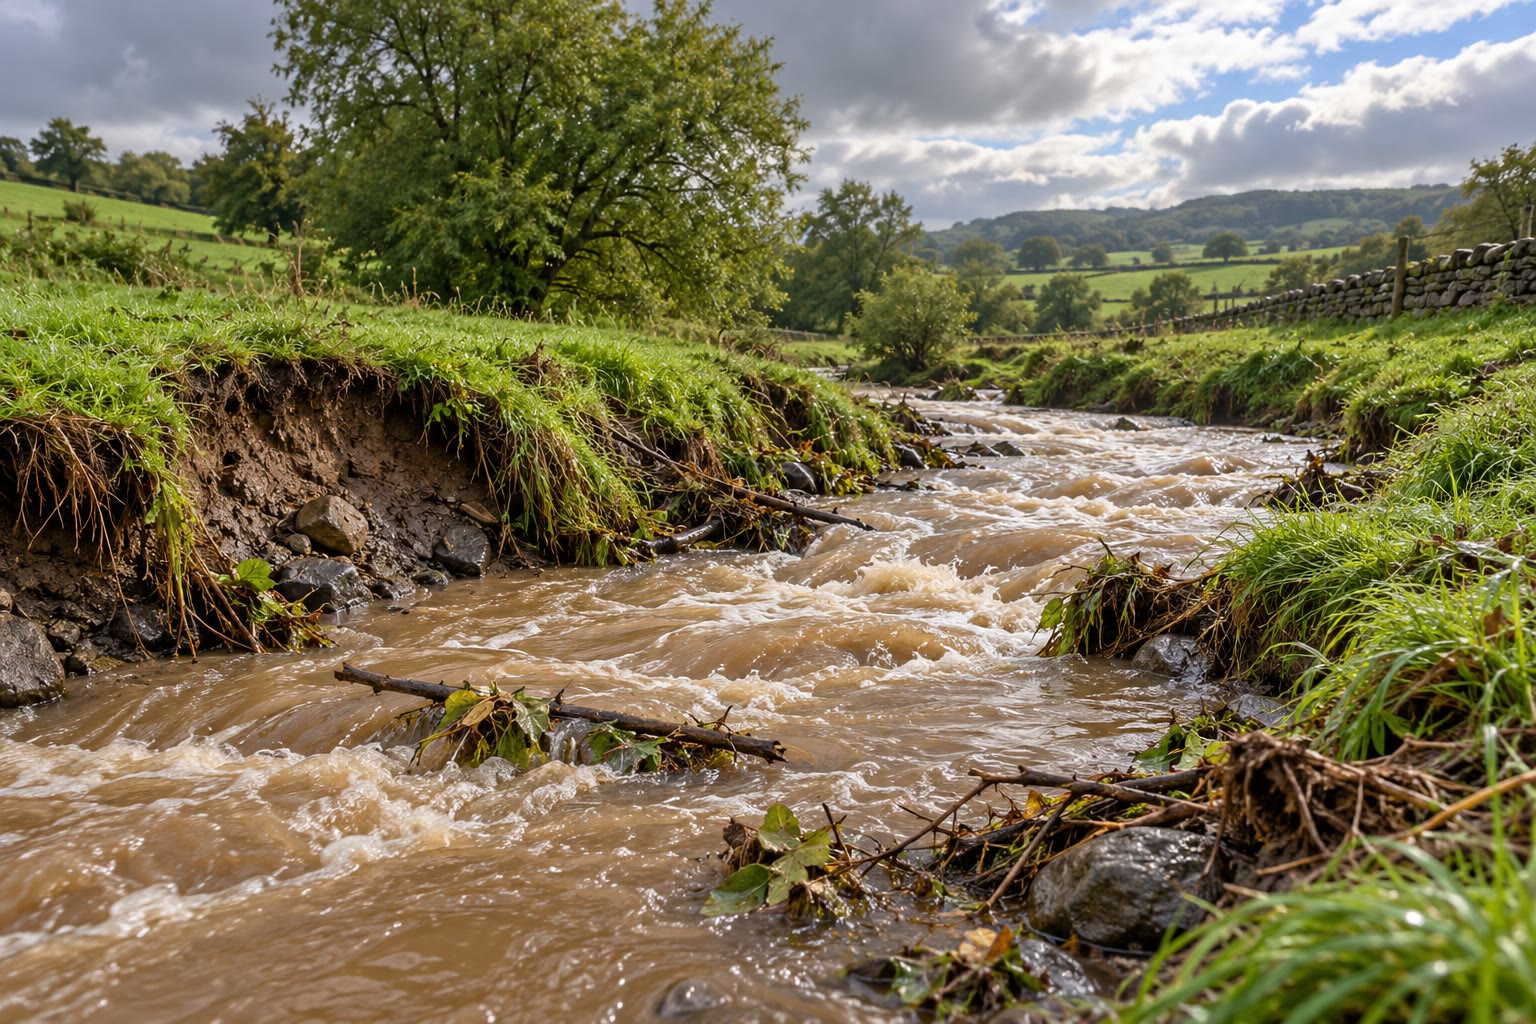
\includegraphics[width=0.5\linewidth]{images/book1/ai/g5-brown-stream.jpg}

{\small तूफ़ान के बाद की सुबह एक धारा: पानी उस \omterm{def:g3:stones-pebbles-sand:sand}{कीचड़} और \omterm{def:g3:stones-pebbles-sand:sand}{रेत} से भूरा है जिसे वह
बहा रहा है।}
\end{omfigure}

\begin{recall}
\omterm{def:g3:stones-pebbles-sand:rock}{चट्टान} पृथ्वी का कठोर पदार्थ है; टुकड़ों में टूटकर वह पत्थर देती है, पानी से गोल
हुए \omterm{def:g3:stones-pebbles-sand:pebble}{कंकड़}, \omterm{def:g3:stones-pebbles-sand:sand}{रेत} जिसके कण हम एक-एक करके देख सकते हैं, और \omterm{def:g3:stones-pebbles-sand:sand}{कीचड़} जिसके कण देखने के
लिए बहुत छोटे हैं (\cref{ch:g3:stones-pebbles-sand})। \omterm{def:g1:landscapes-around-us:water}{नदी} एक लंबी नाली में हर
समय बहती है, ऊँची ज़मीन से नीचे किसी \omterm{def:g1:landscapes-around-us:water}{झील} या \omterm{def:g2:water-on-earth:ocean}{समुद्र} तक
(\cref{ch:g1:landscapes-around-us})। ज़मीन पर गिरने वाली \omterm{def:g4:clouds-rain-snow:precipitation}{बारिश} बहकर धाराओं और
\omterm{def:g1:landscapes-around-us:water}{नदियों} में जाती है, जो पानी को वापस \omterm{def:g2:water-on-earth:ocean}{समुद्र} तक लाती हैं
(\cref{ch:g2:water-on-earth})।
\end{recall}

\section{चट्टान अपनी जगह पर टूटती है}

सबसे कठोर \omterm{def:g3:stones-pebbles-sand:rock}{चट्टान} भी हमेशा नहीं टिकती। जहाँ वह खुले में, धूप, \omterm{def:g4:clouds-rain-snow:precipitation}{बारिश} और पाले के
नीचे पड़ी है, वहाँ वह धीरे-धीरे चटकती और भुरभुराती है।

\begin{definition}[अपक्षय]\label{def:g5:water-shapes-the-land:weathering}
\emph{अपक्षय}\index{अपक्षय} \omterm{def:g3:stones-pebbles-sand:rock}{चट्टान} का अपनी जगह पर धीरे-धीरे टूटना है, पाले से,
पानी से, पौधों की जड़ों से, और गर्मी और ठंड से। \omterm{def:g3:stones-pebbles-sand:rock}{चट्टान} टुकड़ों में टूट जाती है,
पर टुकड़े अपनी जगह पर रहते हैं।
\end{definition}

पाला \omterm{def:g5:water-shapes-the-land:weathering}{अपक्षय} के सबसे मज़बूत औज़ारों में से एक है। \omterm{def:g4:clouds-rain-snow:precipitation}{बारिश} का पानी \omterm{def:g3:stones-pebbles-sand:rock}{चट्टान} की एक पतली
दरार में रिस जाता है। ठंडी रात में वह जम जाता है, और जब पानी जमता है तो वह
थोड़ी ज़्यादा जगह घेरता है: बर्फ़ दरार की दीवारों पर दबाव डालती है और उसे ज़रा-सा
और चौड़ा खोल देती है। अगले दिन बर्फ़ पिघलती है, और पानी अंदर रिसता है, और अगली
रात वह फिर जम जाता है। बहुत-सी सर्दियों के बाद \omterm{def:g3:stones-pebbles-sand:rock}{चट्टान} का एक टुकड़ा टूटकर अलग हो
जाता है।

\begin{omfigure}
\begin{tikzpicture}[x=1cm, y=1cm, font=\scriptsize]
  \foreach \i/\t in {0/{1. बारिश का पानी\\दरार में रिसता है।},
                     4.3/{2. रात में वह जमता है:\\बर्फ़ दरार को\\चौड़ा करती है।},
                     8.6/{3. बहुत-सी सर्दियों बाद\\एक टुकड़ा टूट जाता है।}} {
    \begin{scope}[xshift=\i cm]
      \fill[gray!35] (0,0) rectangle (3.4,2.6);
      \draw[gray!60!black] (0,2.6) -- (3.4,2.6);
      \node[align=center, anchor=north] at (1.7,-0.15) {\t};
    \end{scope}
  }
  % panel 1: thin crack with water
  \fill[white] (1.55,2.6) -- (1.75,0.9) -- (1.85,2.6) -- cycle;
  \fill[blue!45] (1.6,2.2) -- (1.75,0.9) -- (1.83,2.2) -- cycle;
  \draw[gray!60!black] (1.55,2.6) -- (1.75,0.9) -- (1.85,2.6);
  \foreach \x in {1.3,1.7,2.1} \draw[blue!60, ->] (\x,3.3) -- (\x+0.05,2.8);
  \node[blue!60!black] at (0.6,3.1) {बारिश};
  % panel 2: wider crack with ice
  \begin{scope}[xshift=4.3cm]
    \fill[white] (1.45,2.6) -- (1.75,0.75) -- (1.98,2.6) -- cycle;
    \fill[cyan!15] (1.5,2.3) -- (1.75,0.75) -- (1.94,2.3) -- cycle;
    \draw[cyan!50!black] (1.5,2.3) -- (1.75,0.75) -- (1.94,2.3) -- cycle;
    \draw[gray!60!black] (1.45,2.6) -- (1.75,0.75) -- (1.98,2.6);
    \draw[red!70!black, thick, <-] (1.05,1.9) -- (1.5,1.9);
    \draw[red!70!black, thick, ->] (1.98,1.9) -- (2.45,1.9);
    \node[cyan!40!black] at (1.72,3.0) {बर्फ़};
  \end{scope}
  % panel 3: broken block
  \begin{scope}[xshift=8.6cm]
    \fill[white] (1.35,2.6) -- (1.75,0.6) -- (3.4,0.6) -- (3.4,2.6) -- cycle;
    \draw[gray!60!black] (1.35,2.6) -- (1.75,0.6) -- (3.4,0.6);
    \fill[gray!35, draw=gray!60!black, rotate around={-25:(2.9,0.3)}]
      (2.3,0.3) -- (2.4,1.4) -- (3.5,1.35) -- (3.4,0.3) -- cycle;
    \draw[gray!60!black, ->] (2.6,2.2) to[bend left=20] (3.0,1.5);
  \end{scope}
\end{tikzpicture}

{\small पाला \omterm{def:g3:stones-pebbles-sand:rock}{चट्टान} तोड़ता है। पाले की हर रात दरार में जमी बर्फ़ थोड़ा दबाती है;
बहुत-सी सर्दियों के बाद दरार इतनी चौड़ी हो जाती है कि एक टुकड़ा टूटकर अलग हो
जाए।}
\end{omfigure}

पहाड़ों में ऊँचे पर नंगी \omterm{def:g3:stones-pebbles-sand:rock}{चट्टान} की किसी कगार के नीचे पाले से टूटे टुकड़े फिसलते
और लुढ़कते हुए नीचे आते हैं, और नुकीले पत्थरों की एक ढलान में जमा हो जाते हैं।
वे गोल नहीं हैं: अभी किसी पानी ने उन्हें लुढ़काया नहीं है।

\begin{omfigure}
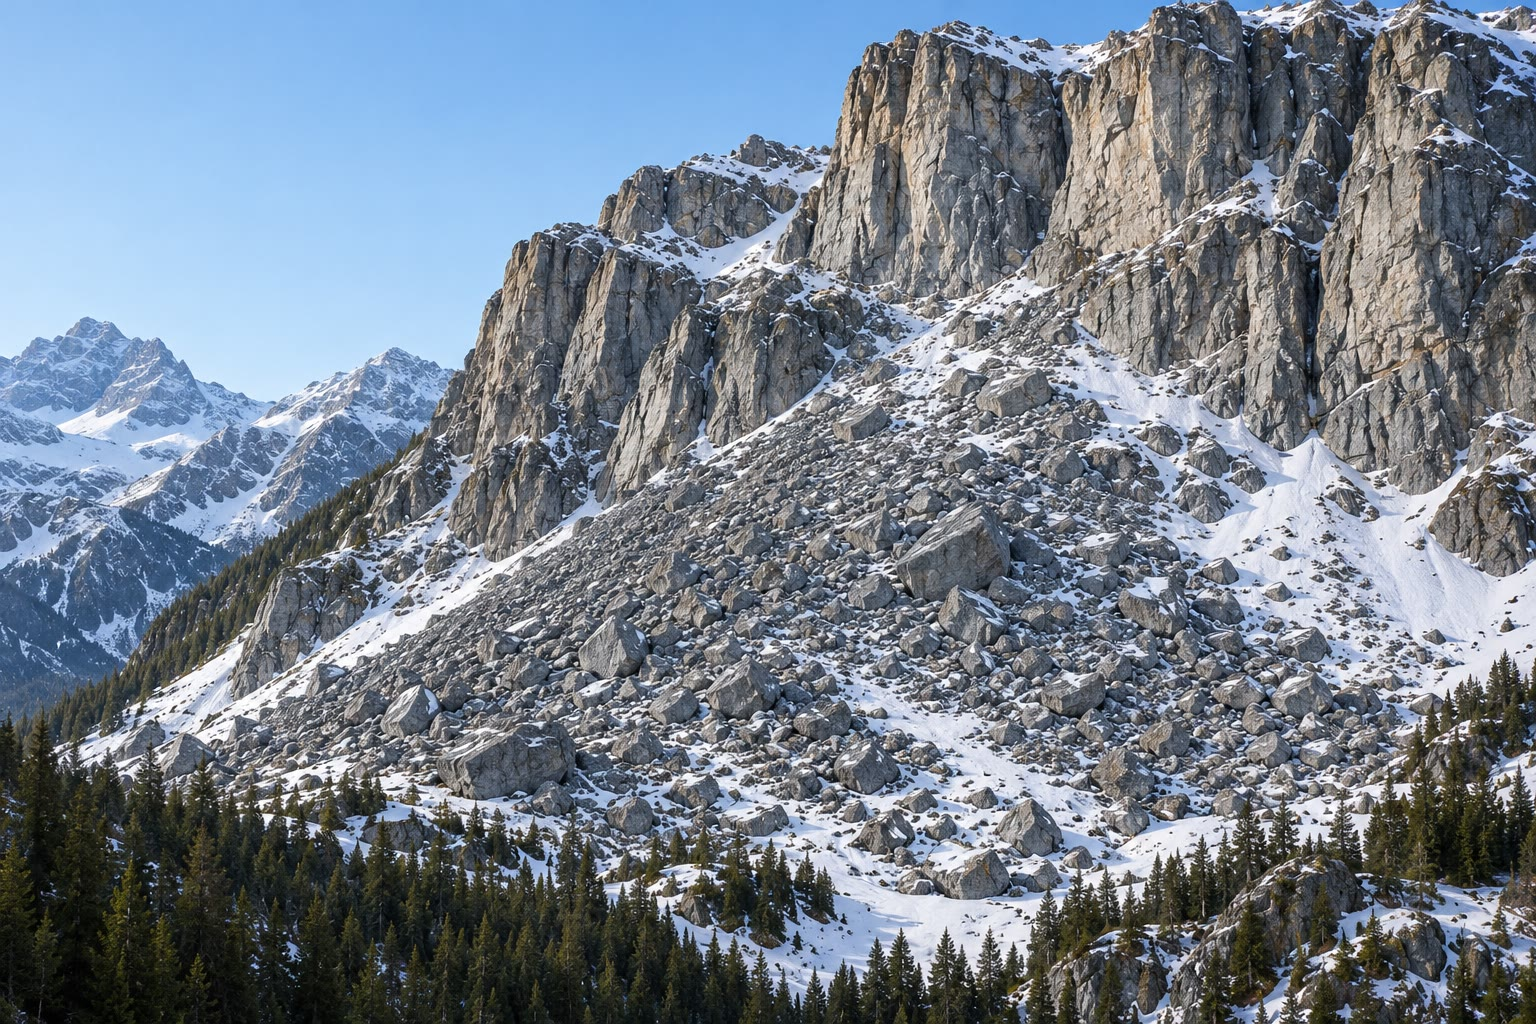
\includegraphics[width=0.5\linewidth]{images/book1/ai/g5-frost-scree.jpg}

{\small पहाड़ की एक कगार के नीचे पाले से टूटे नुकीले किनारों वाले पत्थरों की ढलान,
\omterm{def:g1:landscapes-around-us:landform}{घाटी} के उस पार से दिखती हुई।}
\end{omfigure}

पौधे भी मदद करते हैं। किसी पेड़ की जड़ एक दरार में घुस जाती है और, जैसे-जैसे वह
साल-दर-साल मोटी होती है, \omterm{def:g3:stones-pebbles-sand:rock}{चट्टान} को एक धीमी कील की तरह चीर देती है। \omterm{def:g4:clouds-rain-snow:precipitation}{बारिश} का
पानी ख़ुद भी कुछ \omterm{def:g3:stones-pebbles-sand:rock}{चट्टानों} को धीरे-धीरे नरम करता है और उन्हें चिकनी मिट्टी और \omterm{def:g3:stones-pebbles-sand:sand}{रेत}
में बदल देता है: इसी तरह मिट्टी को उसके खनिज कण मिलते हैं।

\section{पानी टुकड़ों को बहा ले जाता है}

\omterm{def:g3:stones-pebbles-sand:rock}{चट्टान} एक बार टूट जाए, तो टुकड़े हिल सकते हैं। कोई चीज़ उन्हें ढोकर ले जाए, यह ज़रूरी है।

\begin{definition}[अपरदन]\label{def:g5:water-shapes-the-land:erosion}
\emph{अपरदन}\index{अपरदन} ज़मीन का घिसना और \omterm{def:g3:stones-pebbles-sand:rock}{चट्टान} के टुकड़ों का बहकर दूर जाना
है, सबसे बढ़कर बहते पानी से, पर हवा से, बर्फ़ से और \omterm{def:g2:water-on-earth:ocean}{समुद्र} की लहरों से
भी।
\end{definition}

ज़्यादातर काम बहता पानी करता है। \omterm{def:g4:clouds-rain-snow:precipitation}{बारिश} मिट्टी और कणों को ढलानों से धोकर धाराओं
में ले जाती है; धाराएँ अपने ही किनारों से और उखाड़ती हैं, जैसे तूफ़ान के बाद टॉम
और लीना की धारा ने किया। पानी जितना तेज़ बहता है, उतना ज़्यादा वह ढो सकता है, और
उतने ही बड़े टुकड़े हिला सकता है: शांत धारा केवल बारीक \omterm{def:g3:stones-pebbles-sand:sand}{कीचड़} ढोती है; \omterm{def:g5:water-shapes-the-land:flood}{बाढ़} में
आई धारा अपनी तली पर \omterm{def:g3:stones-pebbles-sand:pebble}{कंकड़} और यहाँ तक कि शिलाखंड भी लुढ़काती
है।

रास्ते में पत्थर एक-दूसरे से और तली से टकराते हैं। उनके कोने टूट जाते हैं, और वे
गोल \omterm{def:g3:stones-pebbles-sand:pebble}{कंकड़} बन जाते हैं, फिर छोटे और छोटे कण: \omterm{def:g3:stones-pebbles-sand:sand}{रेत} और
\omterm{def:g3:stones-pebbles-sand:sand}{कीचड़}।

सूखी जगहों में, जहाँ \omterm{def:g3:stones-pebbles-sand:sand}{रेत} को कुछ नहीं थामता, हवा यही काम करती है: वह उसे उड़ाकर
टीलों में जमा करती है। पहाड़ों में और \omterm{def:g3:continents-and-oceans:poles}{ध्रुवों} के पास बर्फ़ अपने भारी वज़न के नीचे
पत्थरों को घसीटती है। \omterm{def:g1:landscapes-around-us:water}{तट} पर लहरें कगारों पर चोट करती हैं और \omterm{def:g2:water-on-earth:ocean}{समुद्र} \omterm{def:g1:landscapes-around-us:water}{तट} के \omterm{def:g3:stones-pebbles-sand:pebble}{कंकड़ों}
को आगे-पीछे लुढ़काती हैं।

\begin{remark}[कितना?]\label{rem:g5:water-shapes-the-land:how-much}
दुनिया की सारी \omterm{def:g1:landscapes-around-us:water}{नदियाँ} मिलकर हर साल 12 अरब टन से ज़्यादा \omterm{def:g3:stones-pebbles-sand:sand}{कीचड़} और \omterm{def:g3:stones-pebbles-sand:sand}{रेत} \omterm{def:g2:water-on-earth:ocean}{समुद्र} तक
लाती हैं। यह हर महीने लगभग एक अरब टन
है।
% ledger: syvitski:modern-flux
\end{remark}

\section{पानी टुकड़ों को नीचे बिठा देता है}

कोई \omterm{def:g1:landscapes-around-us:water}{नदी} अपना बोझ हमेशा नहीं ढो सकती। जहाँ वह धीमी होती है, वहाँ उसमें अपने सबसे
बड़े कणों को हिलाने की ताक़त नहीं रहती, और वे तली पर बैठ जाते हैं।

\begin{definition}[निक्षेपण]\label{def:g5:water-shapes-the-land:deposition}
\emph{निक्षेपण}\index{निक्षेपण} पानी, हवा या बर्फ़ से ढोए गए \omterm{def:g3:stones-pebbles-sand:rock}{चट्टान} के टुकड़ों का
वहाँ नीचे बिछ जाना है, जहाँ वे धीमे होकर रुक जाते हैं।
\end{definition}

सबसे भारी टुकड़े पहले बैठते हैं: \omterm{def:g3:stones-pebbles-sand:pebble}{कंकड़} वहाँ गिरते हैं जहाँ धारा थोड़ी ढीली पड़ती है,
\omterm{def:g3:stones-pebbles-sand:sand}{रेत} वहाँ जहाँ वह और धीमी होती है, और बारीक \omterm{def:g3:stones-pebbles-sand:sand}{कीचड़} केवल वहाँ जहाँ पानी लगभग
ठहरा हो, किसी \omterm{def:g1:landscapes-around-us:water}{झील} में या \omterm{def:g2:water-on-earth:ocean}{समुद्र} में। इसीलिए \omterm{def:g1:landscapes-around-us:water}{नदी} की तली पहाड़ों में \omterm{def:g3:stones-pebbles-sand:pebble}{कंकड़ों} वाली
और \omterm{def:g2:water-on-earth:ocean}{समुद्र} के पास रेतीली या \omterm{def:g3:stones-pebbles-sand:sand}{कीचड़} भरी होती है।

\omterm{def:g5:water-shapes-the-land:weathering}{अपक्षय}, \omterm{def:g5:water-shapes-the-land:erosion}{अपरदन} और \omterm{def:g5:water-shapes-the-land:deposition}{निक्षेपण} एक लंबी यात्रा के तीन क़दम हैं: \omterm{def:g3:stones-pebbles-sand:rock}{चट्टान} अपनी जगह पर
टूटती है, उसके टुकड़े बहकर दूर जाते हैं, और वे कहीं और नीचे बिछ जाते हैं।
धीरे-धीरे पानी \omterm{def:g1:landscapes-around-us:landform}{पर्वतों} को, कण-कण करके, नीचे \omterm{def:g1:landscapes-around-us:landform}{मैदानों} तक और \omterm{def:g2:water-on-earth:ocean}{समुद्र} में ले जाता
है।

\begin{method}[पानी क्या करता है, उसका नाम बताना]\label{met:g5:water-shapes-the-land:naming}
किसी चित्र या कहानी में \omterm{def:g3:stones-pebbles-sand:rock}{चट्टान} के साथ क्या हो रहा है, उसका नाम बताने के लिए तीन
प्रश्न पूछो:
\begin{enumerate}
  \item क्या \omterm{def:g3:stones-pebbles-sand:rock}{चट्टान} टूट रही है, पर टुकड़े वहीं के वहीं रहते हैं?
        वह \emph{\omterm{def:g5:water-shapes-the-land:weathering}{अपक्षय}} है।
  \item क्या टुकड़े घिसकर दूर ले जाए जा रहे हैं? वह
        \emph{\omterm{def:g5:water-shapes-the-land:erosion}{अपरदन}} है।
  \item क्या टुकड़े नीचे बैठकर ढेर बन रहे हैं? वह
        \emph{\omterm{def:g5:water-shapes-the-land:deposition}{निक्षेपण}} है।
\end{enumerate}
\end{method}

\begin{example}[तूफ़ान के बाद की धारा]\label{ex:g5:water-shapes-the-land:stream}
टॉम और लीना की धारा का भूरा पानी अपने किनारों से उखाड़ा \omterm{def:g3:stones-pebbles-sand:sand}{कीचड़} बहा रहा है: वह
\omterm{def:g5:water-shapes-the-land:erosion}{अपरदन} है। एक हफ़्ते बाद धारा फिर साफ़ है, और खेल के मैदान के छोर पर के शांत
कुंड की तली को \omterm{def:g3:stones-pebbles-sand:sand}{कीचड़} की एक पतली परत ढके हुए है:
वह \omterm{def:g5:water-shapes-the-land:deposition}{निक्षेपण} है।
\end{example}

\section{उद्गम से मुहाने तक एक नदी}

हर \omterm{def:g1:landscapes-around-us:water}{नदी} की एक शुरुआत और एक अंत होता है।

\begin{definition}[उद्गम, मुहाना और सहायक नदी]\label{def:g5:water-shapes-the-land:source-mouth}
किसी \omterm{def:g1:landscapes-around-us:water}{नदी} का \emph{उद्गम}\index{उद्गम (नदी का)} वह जगह है जहाँ से वह शुरू होती
है: एक सोता, पिघलता हिमनद, या कोई ऊँची, गीली ज़मीन जहाँ बहुत-सी नन्ही धाराएँ
शुरू होती हैं। उसका \emph{मुहाना}\index{मुहाना (नदी का)} वह जगह है जहाँ वह ख़त्म
होती है, \omterm{def:g2:water-on-earth:ocean}{समुद्र}, किसी \omterm{def:g1:landscapes-around-us:water}{झील} या किसी बड़ी \omterm{def:g1:landscapes-around-us:water}{नदी} में गिरकर।
\emph{सहायक नदी}\index{सहायक नदी} एक छोटी \omterm{def:g1:landscapes-around-us:water}{नदी} है जो किसी बड़ी \omterm{def:g1:landscapes-around-us:water}{नदी} में आकर
मिलती है।
\end{definition}

अपने रास्ते में \omterm{def:g1:landscapes-around-us:water}{नदी} बदलती जाती है। हम उसकी लंबाई को तीन हिस्सों में बाँटते हैं,
उसका ऊपरी, मध्य और निचला मार्ग।

\begin{omfigure}
\begin{tikzpicture}[x=1.15cm, y=1cm, font=\scriptsize]
  % ground
  \fill[brown!25] (0,-0.6) -- plot[domain=0:11, samples=60]
    (\x,{4.6*exp(-\x/2.4)}) -- (11,-0.6) -- cycle;
  % sea
  \fill[blue!20] (11,-0.6) rectangle (12.6,0.02);
  \draw[blue!70!black, line width=1.3pt] plot[domain=0.15:11, samples=60]
    (\x,{4.6*exp(-\x/2.4)});
  \draw[gray] (11,0.02) -- (12.6,0.02);
  \node[blue!50!black] at (11.9,-0.3) {समुद्र};
  % course limits
  \foreach \x in {2.6,6.6} \draw[gray, dashed] (\x,-0.6) -- (\x,5.4);
  \node[align=center, anchor=north] at (1.3,6.3) {\textbf{ऊपरी मार्ग}\\खड़ी ढलान, तेज़,\\V-आकार की घाटी};
  \node[align=center, anchor=north] at (4.6,6.3) {\textbf{मध्य मार्ग}\\हल्की ढलान,\\विसर्प};
  \node[align=center, anchor=north] at (8.8,6.3) {\textbf{निचला मार्ग}\\लगभग समतल, धीमी,\\चौड़ा बाढ़ का मैदान};
  % source and mouth
  \fill[blue!70!black] (0.15,{4.6*exp(-0.15/2.4)}) circle (2pt);
  \node[anchor=east] at (0.05,3.7) {उद्गम};
  \draw[->] (0.05,3.75) -- (0.12,4.15);
  \node[anchor=south] at (11.4,0.75) {मुहाना};
  \draw[->] (11.4,0.75) -- (11.05,0.15);
  % grain sizes
  \node[anchor=north, align=center, text=brown!50!black] at (1.3,-0.7) {शिलाखंड, कंकड़};
  \node[anchor=north, align=center, text=brown!50!black] at (4.6,-0.7) {कंकड़, रेत};
  \node[anchor=north, align=center, text=brown!50!black] at (8.8,-0.7) {रेत, कीचड़};
  \node[anchor=north, align=center, text=brown!50!black] at (11.8,-0.7) {कीचड़};
\end{tikzpicture}

{\small \omterm{def:g5:water-shapes-the-land:source-mouth}{उद्गम} से \omterm{def:g5:water-shapes-the-land:source-mouth}{मुहाने} तक किसी \omterm{def:g1:landscapes-around-us:water}{नदी} की लंबी परिच्छेदिका (ऊँचाइयाँ बहुत खींची गई
हैं)। नीचे: उसकी तली पर क्या पड़ा है।}
\end{omfigure}

अपने \emph{ऊपरी मार्ग} में, पहाड़ों में, \omterm{def:g1:landscapes-around-us:water}{नदी} युवा और खड़ी ढलान वाली होती है। उसका
पानी तेज़ी से नीचे दौड़ता है, तली पर शिलाखंड लुढ़काता है और \omterm{def:g3:stones-pebbles-sand:rock}{चट्टान} में नीचे की
ओर काटता है। वह खड़ी दीवारों वाली एक सँकरी \omterm{def:g1:landscapes-around-us:landform}{घाटी} खोदती है, जिसका आकार अंग्रेज़ी
अक्षर V जैसा होता है।

अपने \emph{मध्य मार्ग} में ढलान हल्की होती है। \omterm{def:g1:landscapes-around-us:water}{नदी} बड़े-बड़े फंदों में एक ओर से
दूसरी ओर झूलती है।

\begin{definition}[विसर्प]\label{def:g5:water-shapes-the-land:meander}
\emph{विसर्प}\index{विसर्प} \omterm{def:g1:landscapes-around-us:water}{नदी} का एक फंदा है जो \omterm{def:g1:landscapes-around-us:landform}{घाटी} की समतल तली पर बल खाता
हुआ चलता है।
\end{definition}

\omterm{def:g5:water-shapes-the-land:meander}{विसर्प} स्थिर नहीं रहता: वह खिसकता है। हर मोड़ के बाहरी ओर पानी तेज़ और गहरा
बहता है: वह किनारे को काटता है, जो एक छोटी कगार बन जाता है। मोड़ के भीतरी ओर
पानी धीरे बहता है: वह \omterm{def:g3:stones-pebbles-sand:sand}{रेत} और \omterm{def:g3:stones-pebbles-sand:pebble}{बजरी} गिराता है, जिनसे एक हल्की ढलान वाला \omterm{def:g1:landscapes-around-us:water}{तट} बनता
है। साल-दर-साल बाहरी किनारा पीछे घिसता है और भीतरी \omterm{def:g1:landscapes-around-us:water}{तट} बढ़ता है, और फंदा और
चौड़ा और चौड़ा झूलता है।

\begin{omfigure}
\begin{tikzpicture}[x=1cm, y=1cm, font=\scriptsize]
  % ---- map view ----
  \fill[green!12] (-0.4,-2.5) rectangle (6.4,2.5);
  % sand on the inner banks (drawn first, the river covers its edge)
  \foreach \c/\s in {1/1, 3/-1, 5/1}
    \fill[yellow!50!orange!45] (\c-0.6,\s*0.5) .. controls (\c,\s*1.5) ..
      (\c+0.6,\s*0.5) .. controls (\c,\s*0.75) .. cycle;
  % the river
  \draw[blue!35, line width=11pt] plot[domain=-0.3:6.3, samples=90]
    (\x,{1.25*sin(\x*90)});
  \draw[blue!70!black, ->, thick] plot[domain=1.6:2.4, samples=10]
    (\x,{1.25*sin(\x*90)});
  \draw[blue!70!black, ->, thick] plot[domain=3.6:4.4, samples=10]
    (\x,{1.25*sin(\x*90)});
  % erosion on the outer banks
  \foreach \c/\s in {1/1, 3/-1, 5/1}
    \foreach \d in {-0.3,0,0.3}
      \draw[red!70!black, thick, ->] (\c+\d,{\s*(1.25*cos(\d*90)+0.22)})
        -- (\c+\d,{\s*(1.25*cos(\d*90)+0.6)});
  \node[red!70!black] at (1,2.2) {अपरदन: बाहरी किनारा};
  \node[red!70!black] at (3,-2.2) {अपरदन: बाहरी किनारा};
  \node[orange!40!black, align=center] (d1) at (1,-0.55) {निक्षेपण:\\भीतरी किनारा};
  \node[orange!40!black, align=center] (d2) at (3,0.55) {निक्षेपण:\\भीतरी किनारा};
  \draw[orange!40!black] (d1.north) -- (1,0.7);
  \draw[orange!40!black] (d2.south) -- (3,-0.7);
  \draw[gray!50!black, dashed] (5,0.15) -- (5,2.3);
  \node[gray!50!black, anchor=north] at (5,0.15) {काट};
  \node[gray!50!black, anchor=east] at (4.95,0.35) {A};
  \node[gray!50!black, anchor=east] at (4.95,2.15) {B};
  \node[anchor=west] at (6.5,0) {ऊपर से दृश्य};
  % ---- cut ----
  \begin{scope}[yshift=-4.1cm, xscale=0.77]
    \fill[brown!25] (-0.4,-1.3) -- (-0.4,0.9) -- (1,0.9) -- (3.6,-0.8)
      .. controls (4.4,-1.05) .. (4.9,-0.9) -- (5.1,0.9) -- (8.4,0.9)
      -- (8.4,-1.3) -- cycle;
    \fill[blue!25] (1.75,0.4) -- (3.6,-0.8) .. controls (4.4,-1.05) .. (4.9,-0.9)
      -- (5.04,0.4) -- cycle;
    \fill[yellow!50!orange!40] (1,0.9) -- (3.6,-0.8) -- (2.6,-0.8) -- cycle;
    \draw[gray!60!black] (-0.4,0.9) -- (1,0.9) -- (3.6,-0.8)
      .. controls (4.4,-1.05) .. (4.9,-0.9) -- (5.1,0.9) -- (8.4,0.9);
    \draw[blue!60!black] (1.75,0.4) -- (5.04,0.4);
    \node[orange!40!black, align=center] at (0.9,-0.4) {भीतरी किनारा:\\धीमा पानी,\\रेतीला तट};
    \node[red!70!black, align=center, anchor=west] at (5.3,-0.3) {बाहरी किनारा:\\तेज़, गहरा पानी,\\छोटी कगार};
    \draw[red!70!black, thick, ->] (4.6,-0.2) -- (5.0,-0.2);
    \node[gray!50!black, anchor=south] at (-0.2,0.9) {A};
    \node[gray!50!black, anchor=south] at (8.2,0.9) {B};
    \node[anchor=west] at (8.45,0) {काट A--B};
  \end{scope}
\end{tikzpicture}

{\small ऊपर से दिखता एक \omterm{def:g5:water-shapes-the-land:meander}{विसर्प}, और धराशायी रेखा A--B के साथ उसकी आड़ी काट।
पानी हर मोड़ के बाहरी किनारे को घिसता है और भीतरी किनारे पर \omterm{def:g3:stones-pebbles-sand:sand}{रेत} गिराता है: फंदा
धीरे-धीरे खिसकता है।}
\end{omfigure}

कभी-कभी दो फंदे इतने पास आ जाते हैं कि \omterm{def:g5:water-shapes-the-land:flood}{बाढ़} के समय \omterm{def:g1:landscapes-around-us:water}{नदी} उनके बीच की ज़मीन की
सँकरी गर्दन को तोड़कर छोटा रास्ता पकड़ लेती है। पुराना फंदा पीछे एक घुमावदार
\omterm{def:g1:landscapes-around-us:water}{झील} बनकर रह जाता है।

\begin{omfigure}
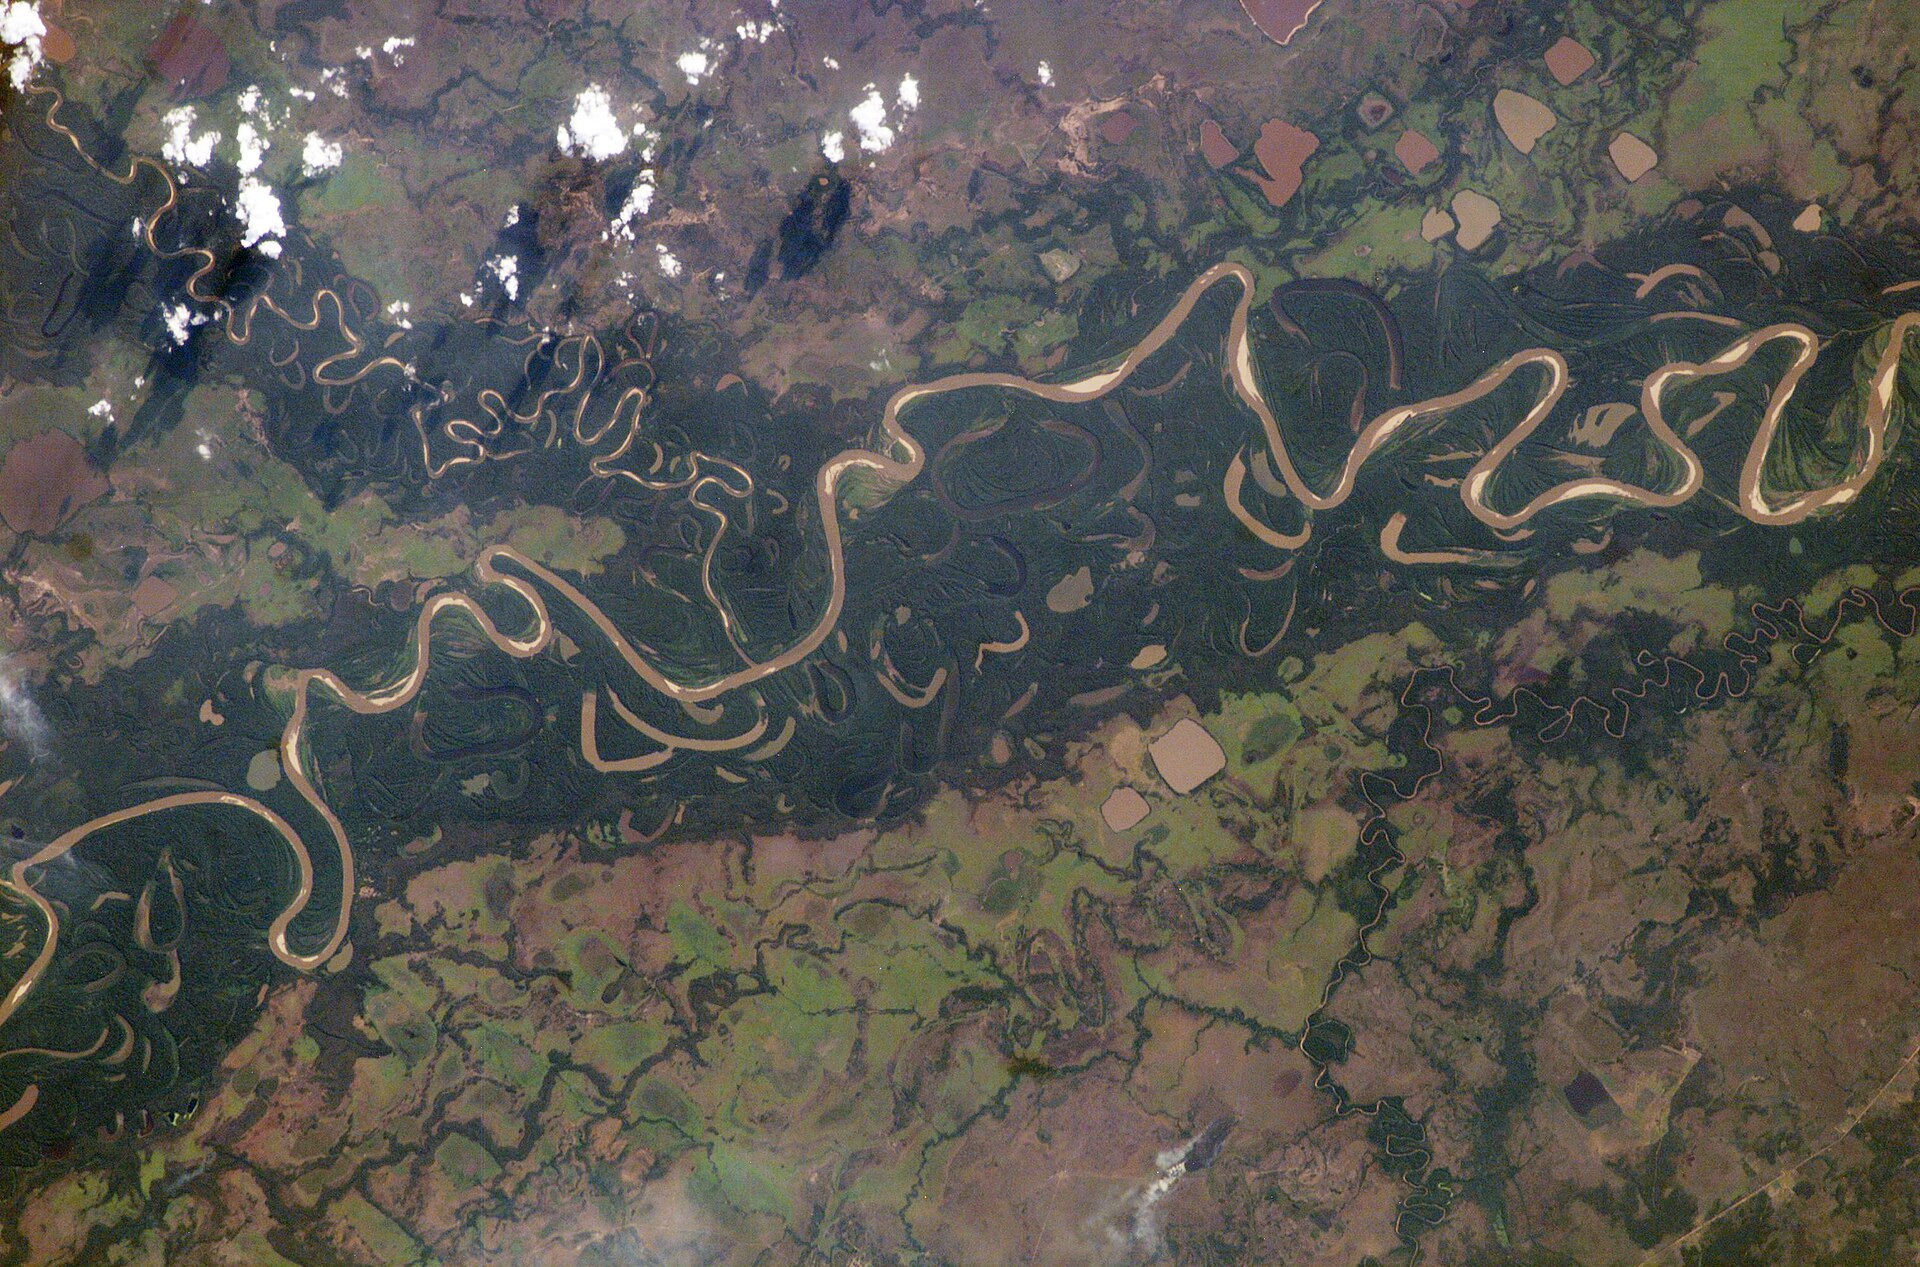
\includegraphics[width=0.52\linewidth]{images/book1/g5-mamore-meanders.jpg}

{\small दक्षिणी अमेरिका में बोलीविया के निचले इलाक़ों में मामोरे \omterm{def:g1:landscapes-around-us:water}{नदी}, अंतरराष्ट्रीय
अंतरिक्ष स्टेशन से दिखती हुई। भूरी \omterm{def:g1:landscapes-around-us:water}{नदी} जंगल के बीच \omterm{def:g5:water-shapes-the-land:meander}{विसर्पों} में बल खाती है।
चित्र: नासा (सार्वजनिक डोमेन)।}\label{fig:g5:water-shapes-the-land:mamore}
% ledger: nasa:mamore-meanders
\end{omfigure}

अपने \emph{निचले मार्ग} में ज़मीन लगभग समतल होती है। \omterm{def:g1:landscapes-around-us:water}{नदी} एक चौड़ी, समतल \omterm{def:g1:landscapes-around-us:landform}{घाटी} की
तली पर धीरे बहती है, जो उसी \omterm{def:g3:stones-pebbles-sand:sand}{कीचड़} और \omterm{def:g3:stones-pebbles-sand:sand}{रेत} से बनी है जिसे उसने बहुत लंबे समय में
ख़ुद नीचे बिछाया है।

\begin{omfigure}
\begin{tikzpicture}[x=1cm, y=1cm, font=\scriptsize]
  % V-shaped valley
  \fill[gray!30] (0,0) -- (0,2.6) -- (0.5,2.6) -- (2.3,0.45) -- (2.7,0.45)
    -- (4.5,2.6) -- (5,2.6) -- (5,0) -- cycle;
  \fill[blue!35] (2.3,0.45) -- (2.4,0.25) -- (2.6,0.25) -- (2.7,0.45) -- cycle;
  \draw[gray!60!black] (0,2.6) -- (0.5,2.6) -- (2.3,0.45) -- (2.4,0.25)
    -- (2.6,0.25) -- (2.7,0.45) -- (4.5,2.6) -- (5,2.6);
  \draw[red!70!black, thick, ->] (2.5,1.9) -- (2.5,0.6);
  \node[red!70!black, anchor=south] at (2.5,1.9) {नीचे काटती है};
  \node[align=center, anchor=north] at (2.5,-0.1) {ऊपरी मार्ग:\\सँकरी V-आकार की घाटी};
  % floodplain
  \begin{scope}[xshift=6cm]
    \fill[gray!30] (0,0) -- (0,2.6) -- (0.6,2.6) -- (1.3,0.9) -- (5.7,0.9)
      -- (6.4,2.6) -- (7,2.6) -- (7,0) -- cycle;
    \fill[brown!25] (1.3,0.9) -- (1.55,0.3) -- (5.45,0.3) -- (5.7,0.9) -- cycle;
    \fill[blue!35] (3.1,0.9) -- (3.25,0.62) -- (3.85,0.62) -- (4,0.9) -- cycle;
    \draw[gray!60!black] (0,2.6) -- (0.6,2.6) -- (1.3,0.9) -- (3.1,0.9)
      -- (3.25,0.62) -- (3.85,0.62) -- (4,0.9) -- (5.7,0.9) -- (6.4,2.6) -- (7,2.6);
    \draw[blue!60!black, dashed] (1.22,1.1) -- (5.78,1.1);
    \node[blue!50!black, anchor=south] at (2.0,1.12) {बाढ़ में};
    \node[brown!50!black] at (2.2,0.55) {कीचड़ और रेत};
    \draw[<->] (1.3,1.75) -- (5.7,1.75);
    \node[anchor=south] at (3.5,1.75) {बाढ़ का मैदान};
    \node[align=center, anchor=north] at (3.5,-0.1) {निचला मार्ग:\\घाटी की चौड़ी, समतल तली};
  \end{scope}
\end{tikzpicture}

{\small \omterm{def:g1:landscapes-around-us:landform}{घाटी} की आड़ी काट, पहाड़ों में और \omterm{def:g2:water-on-earth:ocean}{समुद्र} के पास (एक ही पैमाने पर नहीं)।
\omterm{def:g5:water-shapes-the-land:flood}{बाढ़} में \omterm{def:g1:landscapes-around-us:water}{नदी} अपने पूरे \omterm{def:g5:water-shapes-the-land:flood}{बाढ़} के \omterm{def:g1:landscapes-around-us:landform}{मैदान} पर फैल जाती है।}
\end{omfigure}

आख़िरकार \omterm{def:g1:landscapes-around-us:water}{नदी} अपने \omterm{def:g5:water-shapes-the-land:source-mouth}{मुहाने} पर पहुँचती है। वहाँ पानी लगभग पूरी तरह धीमा हो जाता है,
और \omterm{def:g1:landscapes-around-us:water}{नदी} अपने बोझ का आख़िरी हिस्सा गिरा देती है। जहाँ \omterm{def:g2:water-on-earth:ocean}{समुद्र} की लहरें और ज्वार
उसे पूरा बहा ले जाने के लिए बहुत कमज़ोर हैं, वहाँ \omterm{def:g3:stones-pebbles-sand:sand}{कीचड़} और \omterm{def:g3:stones-pebbles-sand:sand}{रेत} जमा होते जाते हैं,
और नई ज़मीन \omterm{def:g2:water-on-earth:ocean}{समुद्र} में आगे बढ़ती है।

\begin{definition}[डेल्टा]\label{def:g5:water-shapes-the-land:delta}
\emph{डेल्टा}\index{डेल्टा} नई, समतल ज़मीन है जिसे \omterm{def:g1:landscapes-around-us:water}{नदी} अपने \omterm{def:g5:water-shapes-the-land:source-mouth}{मुहाने} पर अपने गिराए
\omterm{def:g3:stones-pebbles-sand:sand}{कीचड़} और \omterm{def:g3:stones-pebbles-sand:sand}{रेत} से बनाती है। \omterm{def:g1:landscapes-around-us:water}{नदी} कई शाखाओं में बँट जाती है जो उस पर फैल जाती हैं,
अक्सर पंखे के आकार में।
\end{definition}

यह नाम यूनानी अक्षर $\Delta$ (\omterm{def:g5:water-shapes-the-land:delta}{डेल्टा}) से आया है, जो एक त्रिभुज है, क्योंकि मिस्र
में नील के \omterm{def:g5:water-shapes-the-land:delta}{डेल्टा} का यही आकार है।

कुछ \omterm{def:g1:landscapes-around-us:water}{नदियाँ} बिना \omterm{def:g5:water-shapes-the-land:delta}{डेल्टा} के ख़त्म होती हैं। जहाँ तेज़ लहरें और ज्वार \omterm{def:g3:stones-pebbles-sand:sand}{कीचड़} को बहा
ले जाते हैं, वहाँ \omterm{def:g1:landscapes-around-us:water}{नदी} एक चौड़े, कीप के आकार के \omterm{def:g5:water-shapes-the-land:source-mouth}{मुहाने} में ख़त्म होती है जहाँ ज्वार
के साथ \omterm{def:g2:water-on-earth:ocean}{समुद्र} अंदर-बाहर आता-जाता है: एक \emph{ज्वारनदमुख}।

\begin{omfigure}
\begin{minipage}[b]{0.55\linewidth}\centering
\begin{tikzpicture}[x=0.68cm, y=0.62cm, font=\scriptsize]
  \fill[blue!20] (-3.6,1.4) rectangle (3.6,3.6);
  \fill[green!15] (-3.6,-1.6) rectangle (3.6,1.4);
  % delta
  \fill[olive!35] (-2.6,1.4) .. controls (-2.2,2.4) and (-1,2.9)
    .. (0,3.0) .. controls (1,2.9) and (2.2,2.4) .. (2.6,1.4) -- cycle;
  \draw[gray!60!black] (-3.6,1.4) -- (-2.6,1.4) .. controls (-2.2,2.4) and
    (-1,2.9) .. (0,3.0) .. controls (1,2.9) and (2.2,2.4) .. (2.6,1.4) -- (3.6,1.4);
  \draw[gray!60!black, dashed] (-2.6,1.4) -- (2.6,1.4);
  % river and branches
  \draw[blue!60!black, line width=2pt] (0,-1.6) .. controls (0.3,-0.5) .. (0,0.9);
  \foreach \e in {-1.9,-0.9,0.2,1.2,2.0}
    \draw[blue!60!black, line width=1pt] (0,0.9) .. controls (\e*0.3,1.6) ..
      (\e,{2.95-0.3*\e*\e});
  % mud plume
  \fill[brown!30, opacity=0.5] (-1.3,3.05) .. controls (0,3.6) .. (1.3,3.0)
    .. controls (0,3.25) .. cycle;
  \node[align=center] at (-2.8,3.1) {समुद्र};
  \node[anchor=west, brown!50!black] at (1.35,3.25) {कीचड़};
  \node[anchor=west, align=left] at (3.7,2.4) {डेल्टा:\\नई ज़मीन};
  \draw (3.7,2.4) -- (2.0,2.2);
  \node[anchor=west, align=left, gray!50!black] at (3.7,1.0) {पुराना\\तट};
  \draw[gray!50!black] (3.7,1.0) -- (2.3,1.4);
  \node[anchor=west] at (0.35,-1.1) {नदी};
\end{tikzpicture}
\end{minipage}\hfill
\begin{minipage}[b]{0.3\linewidth}\centering
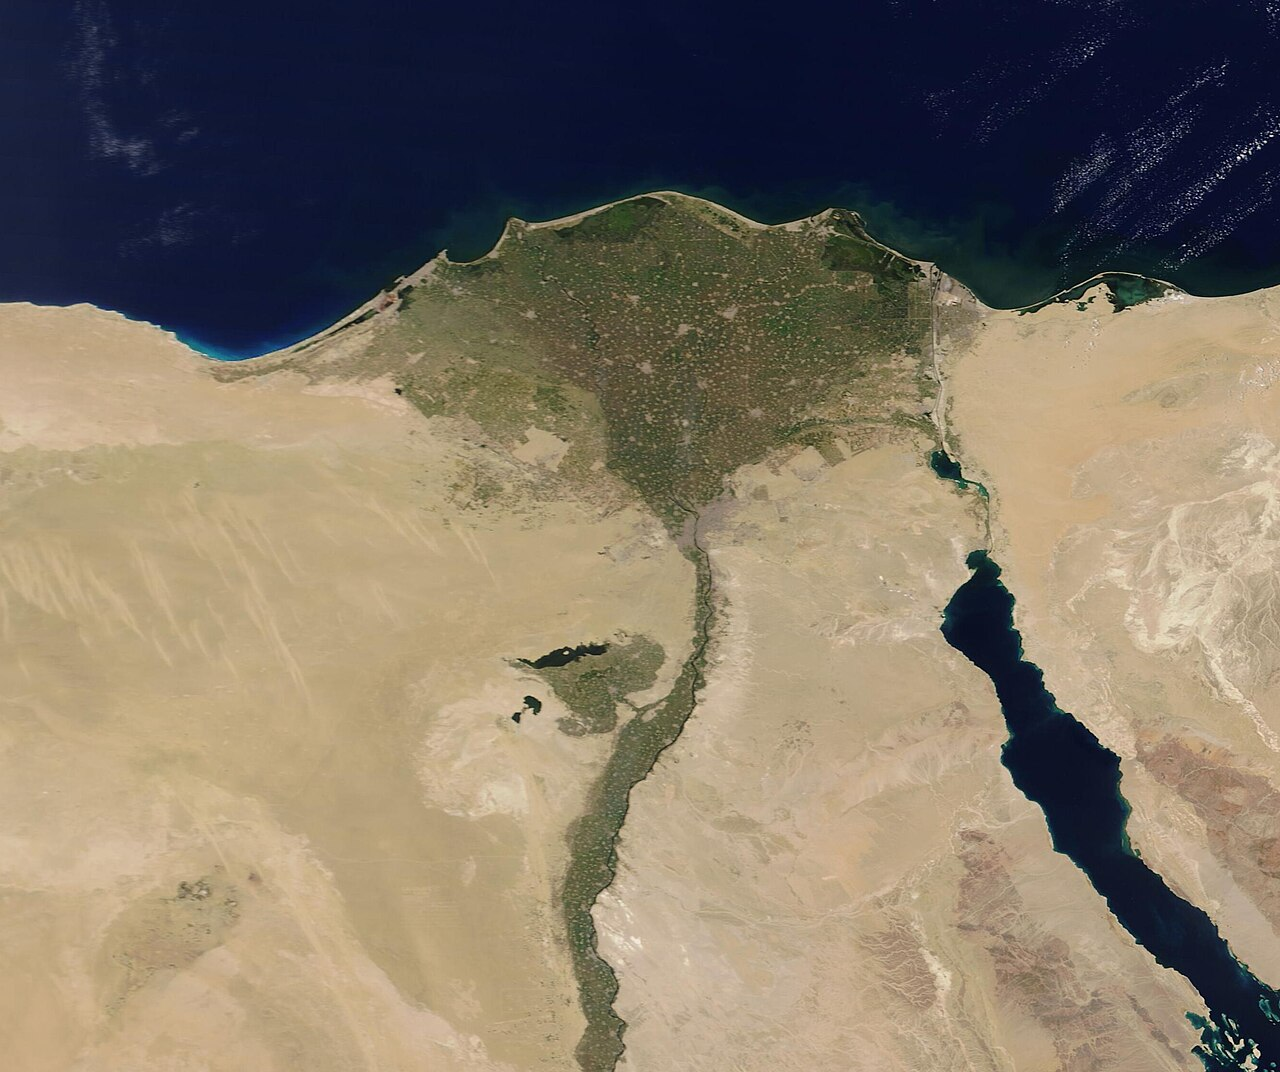
\includegraphics[width=\linewidth]{images/book1/g5-nile-delta-modis.jpg}
\end{minipage}

{\small बाएँ: ऊपर से दिखता एक \omterm{def:g5:water-shapes-the-land:delta}{डेल्टा}; शाखाओं के गिराए \omterm{def:g3:stones-pebbles-sand:sand}{कीचड़} और \omterm{def:g3:stones-pebbles-sand:sand}{रेत} पुराने \omterm{def:g1:landscapes-around-us:water}{तट} के
आगे नई ज़मीन बनाते हैं। दाएँ: मिस्र में नील का \omterm{def:g5:water-shapes-the-land:delta}{डेल्टा}, एक उपग्रह से (\omterm{def:g2:water-on-earth:ocean}{समुद्र}
ऊपर): रेगिस्तान के बीच \omterm{def:g1:landscapes-around-us:water}{नदी} के \omterm{def:g3:stones-pebbles-sand:sand}{कीचड़} पर खेतों का एक हरा पंखा। चित्र: नासा
(सार्वजनिक
डोमेन)।}
% ledger: nasa:nile-delta-modis
\end{omfigure}

\section{बाढ़}

\omterm{def:g4:clouds-rain-snow:precipitation}{बारिश} के लंबे दिनों के बाद, या जब वसंत में \omterm{def:g4:clouds-rain-snow:precipitation}{हिम} तेज़ी से पिघलता है, किसी \omterm{def:g1:landscapes-around-us:water}{नदी} को
उससे ज़्यादा पानी मिलता है जितना उसकी नाली सँभाल सकती है।

\begin{definition}[बाढ़ और बाढ़ का मैदान]\label{def:g5:water-shapes-the-land:flood}
\emph{बाढ़}\index{बाढ़} तब आती है जब पानी उस ज़मीन को ढक लेता है जो आमतौर पर
सूखी रहती है। \omterm{def:g1:landscapes-around-us:water}{नदी} में बाढ़ तब आती है जब वह अपने किनारों से ऊपर उठकर अपने दोनों
ओर की समतल ज़मीन पर फैल जाती है। वह समतल ज़मीन, जिसे \omterm{def:g1:landscapes-around-us:water}{नदी} समय-समय पर ढकती है,
उसका \emph{बाढ़ का मैदान}\index{बाढ़ का मैदान} है।
\end{definition}

\begin{omfigure}
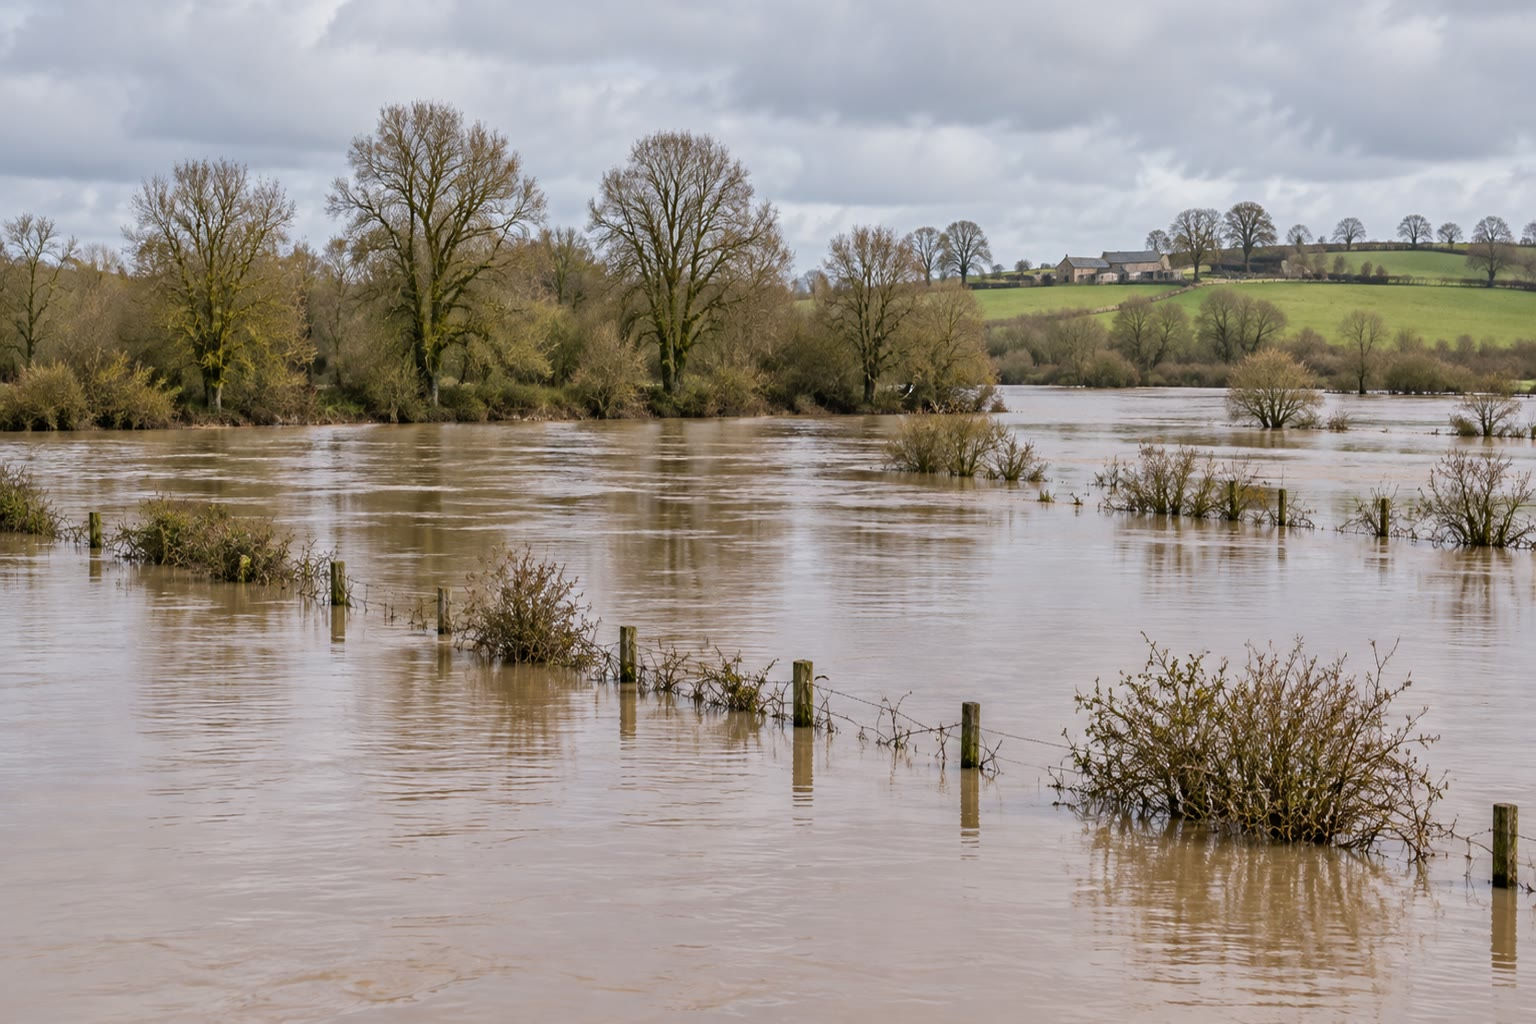
\includegraphics[width=0.5\linewidth]{images/book1/ai/g5-flooded-meadow.jpg}

{\small कई दिनों की \omterm{def:g4:clouds-rain-snow:precipitation}{बारिश} के बाद \omterm{def:g5:water-shapes-the-land:flood}{बाढ़} के पानी में डूबा एक चरागाह। पेड़ों की कतार
\omterm{def:g1:landscapes-around-us:water}{नदी} के सामान्य किनारे को दिखाती है; खेत-घर ऊँची ज़मीन पर खड़ा है।}
\end{omfigure}

\omterm{def:g5:water-shapes-the-land:flood}{बाढ़} लाने वाली \omterm{def:g1:landscapes-around-us:water}{नदी} कोई अजीब काम नहीं कर रही: वह वही कर रही है जो \omterm{def:g1:landscapes-around-us:water}{नदियाँ} हमेशा
से करती आई हैं। \omterm{def:g5:water-shapes-the-land:flood}{बाढ़ का मैदान} उसका इलाक़ा है। असल में \omterm{def:g1:landscapes-around-us:water}{नदी} ने ही उसे बनाया है: हर
\omterm{def:g5:water-shapes-the-land:flood}{बाढ़} खेतों पर \omterm{def:g3:stones-pebbles-sand:sand}{कीचड़} की एक पतली परत छोड़ जाती है, इसीलिए \omterm{def:g5:water-shapes-the-land:flood}{बाढ़} के \omterm{def:g1:landscapes-around-us:landform}{मैदानों} की मिट्टी
इतनी उपजाऊ होती है। बहुत पहले मिस्र के किसान
नील की सालाना \omterm{def:g5:water-shapes-the-land:flood}{बाढ़} का इंतज़ार करते थे, जो उनके खेतों को सींचती थी और उन्हें नया
\omterm{def:g3:stones-pebbles-sand:sand}{कीचड़} लाती थी।

पर \omterm{def:g5:water-shapes-the-land:flood}{बाढ़} के \omterm{def:g1:landscapes-around-us:landform}{मैदान} पर रहने वाले लोगों के लिए \omterm{def:g5:water-shapes-the-land:flood}{बाढ़} ख़तरनाक है। उस पर बने घरों में
पानी भर सकता है, और \omterm{def:g5:water-shapes-the-land:flood}{बाढ़} का तेज़ पानी कारों और लोगों को बहा ले जा सकता है।
समझदार शहर ऊँची ज़मीन पर बनता है और \omterm{def:g5:water-shapes-the-land:flood}{बाढ़} के \omterm{def:g1:landscapes-around-us:landform}{मैदान} को खेतों, चरागाहों और
उद्यानों के लिए छोड़ देता है। \cref{ch:g5:natural-hazards} में
हम देखेंगे कि लोग \omterm{def:g5:water-shapes-the-land:flood}{बाढ़} के लिए कैसे तैयारी करते हैं और सुरक्षित रहते हैं।

\begin{safety}
\omterm{def:g5:water-shapes-the-land:flood}{बाढ़} के पानी में कभी मत चलो, साइकिल मत चलाओ या खेलो मत, और \omterm{def:g5:water-shapes-the-land:flood}{बाढ़} में आई \omterm{def:g1:landscapes-around-us:water}{नदी} के पास
कभी मत जाओ: पानी जितना दिखता है उससे ज़्यादा ताक़तवर और गहरा होता है, और वह गड्ढे
और खुली नालियाँ छिपा सकता है। जब तक ज़िम्मेदार बड़े यह न कहें कि अब सुरक्षित है,
तब तक दूर रहो।
\end{safety}

\section{अभ्यास}

\begin{exercise}[$\star$]\label{exo:g5:water-shapes-the-land:1}
प्रक्रिया का नाम बताओ: \omterm{def:g5:water-shapes-the-land:weathering}{अपक्षय}, \omterm{def:g5:water-shapes-the-land:erosion}{अपरदन} या \omterm{def:g5:water-shapes-the-land:deposition}{निक्षेपण}?
\begin{enumerate}
  \item[(क)] किसी \omterm{def:g1:landscapes-around-us:landform}{पर्वत} पर एक दरार में जमी बर्फ़ एक \omterm{def:g3:stones-pebbles-sand:rock}{चट्टान} को चीर देती है।
  \item[(ख)] \omterm{def:g5:water-shapes-the-land:flood}{बाढ़} में आई एक \omterm{def:g1:landscapes-around-us:water}{नदी} अपने किनारों से \omterm{def:g3:stones-pebbles-sand:sand}{रेत} बहा ले जाती है।
  \item[(ग)] एक शांत \omterm{def:g1:landscapes-around-us:water}{झील} की तली पर \omterm{def:g3:stones-pebbles-sand:sand}{कीचड़} की एक परत बैठ जाती है।
  \item[(घ)] एक पेड़ की जड़ पत्थर की एक दीवार को चीर देती है।
\end{enumerate}
\end{exercise}

\begin{exercise}[$\star$]\label{exo:g5:water-shapes-the-land:2}
\omterm{def:g1:landscapes-around-us:water}{नदी} का \omterm{def:g5:water-shapes-the-land:source-mouth}{उद्गम} क्या है? उसका \omterm{def:g5:water-shapes-the-land:source-mouth}{मुहाना} क्या है? \omterm{def:g5:water-shapes-the-land:source-mouth}{सहायक नदी} क्या है?
\end{exercise}

\begin{exercise}[$\star$]\label{exo:g5:water-shapes-the-land:3}
\omterm{def:g1:landscapes-around-us:water}{नदी} के इन हिस्सों को \omterm{def:g5:water-shapes-the-land:source-mouth}{उद्गम} से \omterm{def:g2:water-on-earth:ocean}{समुद्र} तक के क्रम में लगाओ: \omterm{def:g5:water-shapes-the-land:meander}{विसर्प}; \omterm{def:g5:water-shapes-the-land:delta}{डेल्टा};
सँकरी V-आकार की \omterm{def:g1:landscapes-around-us:landform}{घाटी}; \omterm{def:g5:water-shapes-the-land:source-mouth}{उद्गम}।
\end{exercise}

\begin{exercise}[$\star$]\label{exo:g5:water-shapes-the-land:4}
सही या ग़लत? समझाओ।
\begin{enumerate}
  \item[(क)] कठोर \omterm{def:g3:stones-pebbles-sand:rock}{चट्टान} कभी नहीं बदलती।
  \item[(ख)] तेज़ \omterm{def:g1:landscapes-around-us:water}{नदी} धीमी \omterm{def:g1:landscapes-around-us:water}{नदी} से बड़े पत्थर ढो सकती है।
  \item[(ग)] सबसे बारीक \omterm{def:g3:stones-pebbles-sand:sand}{कीचड़} सबसे पहले, \omterm{def:g5:water-shapes-the-land:source-mouth}{उद्गम} के पास, बैठता है।
\end{enumerate}
\end{exercise}

\begin{exercise}[$\star$]\label{exo:g5:water-shapes-the-land:5}
यहाँ ऊपर से दिखता किसी \omterm{def:g1:landscapes-around-us:water}{नदी} का एक मोड़ है।

\begin{center}
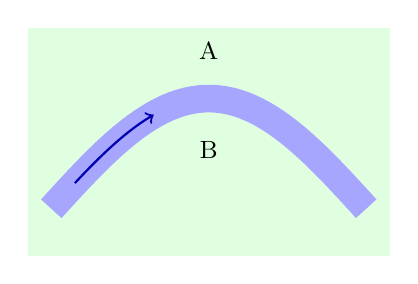
\begin{tikzpicture}[x=1cm, y=1cm, font=\small]
  \fill[green!12] (-0.3,-0.6) rectangle (4.3,2.3);
  \draw[blue!35, line width=10pt] plot[domain=0:4, samples=50]
    (\x,{1.4*sin(\x*45)});
  \draw[blue!70!black, ->, thick] plot[domain=0.3:1.3, samples=20]
    (\x,{1.4*sin(\x*45)});
  \node at (2,2.0) {A};
  \node at (2,0.75) {B};
\end{tikzpicture}
\end{center}
\omterm{def:g1:landscapes-around-us:water}{नदी} किस किनारे पर, A या B, ज़मीन को घिसती है? किस किनारे पर वह
\omterm{def:g3:stones-pebbles-sand:sand}{रेत} गिराती है?
\end{exercise}

\begin{exercise}[$\star$]\label{exo:g5:water-shapes-the-land:6}
पहाड़ों में \omterm{def:g1:landscapes-around-us:water}{नदी} की तली बड़े पत्थरों से ढकी है। \omterm{def:g2:water-on-earth:ocean}{समुद्र} के पास वह \omterm{def:g3:stones-pebbles-sand:sand}{रेत} और \omterm{def:g3:stones-pebbles-sand:sand}{कीचड़}
से ढकी है। क्यों?
\end{exercise}

\begin{exercise}[$\star\star$]\label{exo:g5:water-shapes-the-land:7}
एक \omterm{def:g1:landscapes-around-us:water}{नदी} 600 किलोमीटर लंबी है। उसका ऊपरी मार्ग उसकी लंबाई का पहला
$\frac{1}{6}$ है, और उसका मध्य मार्ग उसके बाद का
$\frac{1}{2}$।
\begin{enumerate}
  \item[(क)] ऊपरी मार्ग कितना लंबा है? मध्य मार्ग?
  \item[(ख)] निचला मार्ग कितना लंबा है? वह \omterm{def:g1:landscapes-around-us:water}{नदी} का कौन-सा भिन्न
        है?
\end{enumerate}
\end{exercise}

\begin{exercise}[$\star\star$]\label{exo:g5:water-shapes-the-land:8}
अंतरिक्ष स्टेशन से दिखती मामोरे \omterm{def:g1:landscapes-around-us:water}{नदी} का फ़ोटो, पृष्ठ~\pageref{fig:g5:water-shapes-the-land:mamore} पर, फिर से देखो। मोड़ों के भीतरी ओर
के हल्के रंग के धब्बे क्या हैं? \omterm{def:g1:landscapes-around-us:water}{नदी} के बगल की गहरे रंग की घुमावदार \omterm{def:g1:landscapes-around-us:water}{झीलें} क्या हैं? वे
कैसे बनीं?
\end{exercise}

\begin{exercise}[$\star\star$]\label{exo:g5:water-shapes-the-land:9}
एक शहर अपनी \omterm{def:g1:landscapes-around-us:water}{नदी} के बगल के समतल हरे चरागाहों में एक नया स्कूल बनाना चाहता है,
क्योंकि वहाँ की ज़मीन समतल और सस्ती है। तुम नगर परिषद को क्या बताओगे?
\emph{\omterm{def:g5:water-shapes-the-land:flood}{बाढ़}} और \emph{\omterm{def:g5:water-shapes-the-land:flood}{बाढ़ का मैदान}} शब्दों का प्रयोग करो।
\end{exercise}

\begin{exercise}[$\star\star$]\label{exo:g5:water-shapes-the-land:10}
दुनिया की \omterm{def:g1:landscapes-around-us:water}{नदियाँ} हर साल लगभग 12 अरब टन \omterm{def:g3:stones-pebbles-sand:sand}{कीचड़} और \omterm{def:g3:stones-pebbles-sand:sand}{रेत} \omterm{def:g2:water-on-earth:ocean}{समुद्र} तक लाती
हैं।
\begin{enumerate}
  \item[(क)] यह औसतन हर महीने कितने टन हुआ?
  \item[(ख)] एक बड़ा ट्रक 10 टन ढोता है। एक महीने का \omterm{def:g3:stones-pebbles-sand:sand}{कीचड़} और \omterm{def:g3:stones-pebbles-sand:sand}{रेत} ढोने में ट्रक
        के कितने फेरे लगेंगे?
\end{enumerate}
\end{exercise}

\begin{exercise}[$\star\star\star$]\label{exo:g5:water-shapes-the-land:11}
\omterm{def:g3:stones-pebbles-sand:sand}{रेत} के एक कण की कहानी सुनाओ। वह किसी \omterm{def:g1:landscapes-around-us:landform}{पर्वत} पर ऊँचे पर एक \omterm{def:g3:stones-pebbles-sand:rock}{चट्टान} के हिस्से के रूप में
शुरू होता है, और बहुत वर्षों बाद एक \omterm{def:g5:water-shapes-the-land:delta}{डेल्टा} में ख़त्म होता है। \emph{\omterm{def:g5:water-shapes-the-land:weathering}{अपक्षय}},
\emph{\omterm{def:g5:water-shapes-the-land:erosion}{अपरदन}} और \emph{\omterm{def:g5:water-shapes-the-land:deposition}{निक्षेपण}} शब्दों का प्रयोग करो, और बताओ कि \omterm{def:g1:landscapes-around-us:water}{नदी} के ऊपरी, मध्य
और निचले मार्ग में कण के साथ क्या होता है।
\end{exercise}
